\documentclass[a4paper, 12pt]{article}
\usepackage{cmap}
\usepackage[warn]{mathtext}
\usepackage[T2A]{fontenc}
\usepackage[utf8]{inputenc}
\usepackage{graphicx}
\usepackage{amssymb}
\usepackage{amsmath}
\usepackage{wrapfig}
\usepackage{siunitx}
\graphicspath{image/}
\title{Измерение модуля Юнга методом акустического резонанса}
\author{Шакиров Тимур Тагирович}
\date{Декабрь 2021}
\renewcommand{\figurename}{Рис.}
\begin{document}

\maketitle

\textbf{Цель работы:} Исследовать явление акустического резонанса в тонком стержне, измерить скорость распространения продольных звуковых колебаний в тонких стержнях из различных материалов. Измерить модуль Юнга различных материалов.

\vspace{1cm}

\textbf{В работе используются:} генератор звуковых частот, частотометр, осцилограф, э/м излучатель и приемник колебаний, набор стержней.

\vspace{1cm}

\section*{Теория.}
Для элемента среды верно:
\begin{equation}
    \sigma=\varepsilon E
\end{equation}
В тонком стержне выполняется равенство:
\begin{equation}
    \frac{\partial^2\xi}{\partial t^2}=\frac{E}{\rho}\frac{\partial^2\xi}{\partial x^2}=u^2\frac{\partial^2\xi}{\partial x^2}
\end{equation}
Произвольная функция $\phi(x\pm ut)$ --- решение уравнения выше.
А общее решение этого уравнения представляется в виде $\phi_1(x+ut)+\phi_2(x-ut)$.\\
В случае гармонического возбуждения с частотой $f$: 
\begin{equation}
\xi(x,t)=A_1 sin(\omega t-kx+\varphi_1)+A_2 sin(\omega t+kx+\varphi_2)
\end{equation}
$\omega=2\pi f$, $k=\frac{2\pi}{\lambda}$, $\lambda$ --- длина волны.\\
Если концы стержня не закреплены, то $A_1=A_2$, $\varphi_1=\varphi_2$.\\
Тогда $\xi(x,t)=2A cos(kx)sin(\omega t+\varphi)$ --- уравнение гармонической стоячей волны.\\
Из граничного условия($\sigma_L=0$) получим, что $sin(kL)=0$, откуда получим условие на $\lambda$: в длине стержня должно укладываться целое число полуволн. Допустимые значения частот $f_n=n\frac{u}{2L}$ называют собсвтенными частотами колебаний. Выразив $u$, получим $u=2L\frac{f_n}{n}$.
\section*{Ход работы}
\begin{itemize}
    \item Настроили осцилограф, генератор, разместили стержень на подставку, установили источник и приемник сигнала.
    \item Оценили частоту первого резонанса в стержнях, зная, что $u_m\approx$
    \item  В режиме X-Y осцилографа нашли первые 3 гармоники стержней из меди, стали, дюраля. Результаты измерений внесли в таблицу.
    \begin{table}[h]
        \centering
        \begin{tabular}{|c|ccc|}
        \hline
        №& 1& 2& 3\\ \hline
        $f_m\text{, Гц}$& 3251.7&  6465.2& 9755.0\\ 
        $f_s\text{, Гц}$& 4117.6& 8235.4& 12354.9\\
        $f_d\text{, Гц}$& 4261.4& 8521.2& 12785.1\\ \hline
        \end{tabular}
    \end{table}\\
    При повторении экспериментов значение резонансной частоты не менялось, так что считаем $\sigma^{\text{сл}}_f \ll\sigma^{\text{сист}}_f=0.1\text{ Гц}$.\\
    $\sigma_f=0.1\text{ Гц}$
    \item Определили плотность материалов. Для этого измерили геометрические размеры и массы образцов материалов. Результаты привели ниже:
    \begin{table}[h]
        \centering
        \begin{tabular}{|c|cccc|}
        \hline
        №& 1& 2& 3& $D_{ср}$\\
        \hline
        $D_m$& 1.20& 1.20& 1.20& 1.20\\
        $D_s$& 1.22& 1.22& 1.23& 1.22\\
        $D_d$& 1.16& 1.17& 1.17& 1.17\\
        \hline
        \end{tabular}
    \end{table}\\
    $\sigma^{\text{сл}}_D \approx\sigma^{\text{сист}}_D=0.01\text{ см}$.\\
    $\sigma_D=0.01\text{ см}$
    \begin{table}[h!]
        \centering
        \begin{tabular}{|c|cccc|c|}
        \hline
        №& D, мм& l, мм& m, г& $\rho$, $\frac{кг}{м^3}$& $\sigma_{\rho}$, $\frac{кг}{м^3}$\\
        \hline
        Медь& 12.0& 39.7& 39.42& 8780& 140\\
        Сталь& 12.2& 41.3& 37.11& 7680& 120\\
        Дюраль& 11.7& 40.1& 11.80& 2730& 50\\
        \hline
        \end{tabular}
    \end{table}\\
    $\sigma_{\rho}=\rho\sqrt{\varepsilon_{m}^2+\varepsilon_{l}^2+4\varepsilon_{D}^2}$\\
    \item Построили графики $f(n)$ для разных материалов, наилучшие прямые этих графиков(смотреть в приложении). Из графиков вычислили величину $\frac{u}{2L}$, из которой определили $u$, $E$.\\
    \begin{table}[h]
        \centering
        \begin{tabular}{|c|ccc|}
        \hline
        №& 1& 2& 3\\
        \hline
        $u$, $\frac{м}{с}$&3900& 4940& 5110\\
        $\sigma_u$, $\frac{м}{с}$& 120& 20& 40\\
        $E$, $ГПа$& 133& 187&   71\\
        $\sigma_E$, $ГПа$& 4& 1& 1\\
        $E_{табл}$, $ГПа$& 110& 190—210&   74\\
        \hline
        \end{tabular}
    \end{table}\\
    $\sigma_u=2L\frac{1}{\sqrt{3}}\sqrt{\frac{\Bar{f_n^2}}{\Bar{n^2}}-\frac{f_n}{n}^2}$\\
    $\sigma_{E}=E\varepsilon_E=E\varepsilon_u$\\
\end{itemize}
С помощью явления акустического резонанса мы с хорошей точностью сумели измерить модули Юнга различных веществ. Небольшое несоответствие полученных значений с табличными скорее всего связаны с несовершенством источника и приемника сигналов.\newpage
\section*{Приложение}
\begin{figure}[h]
    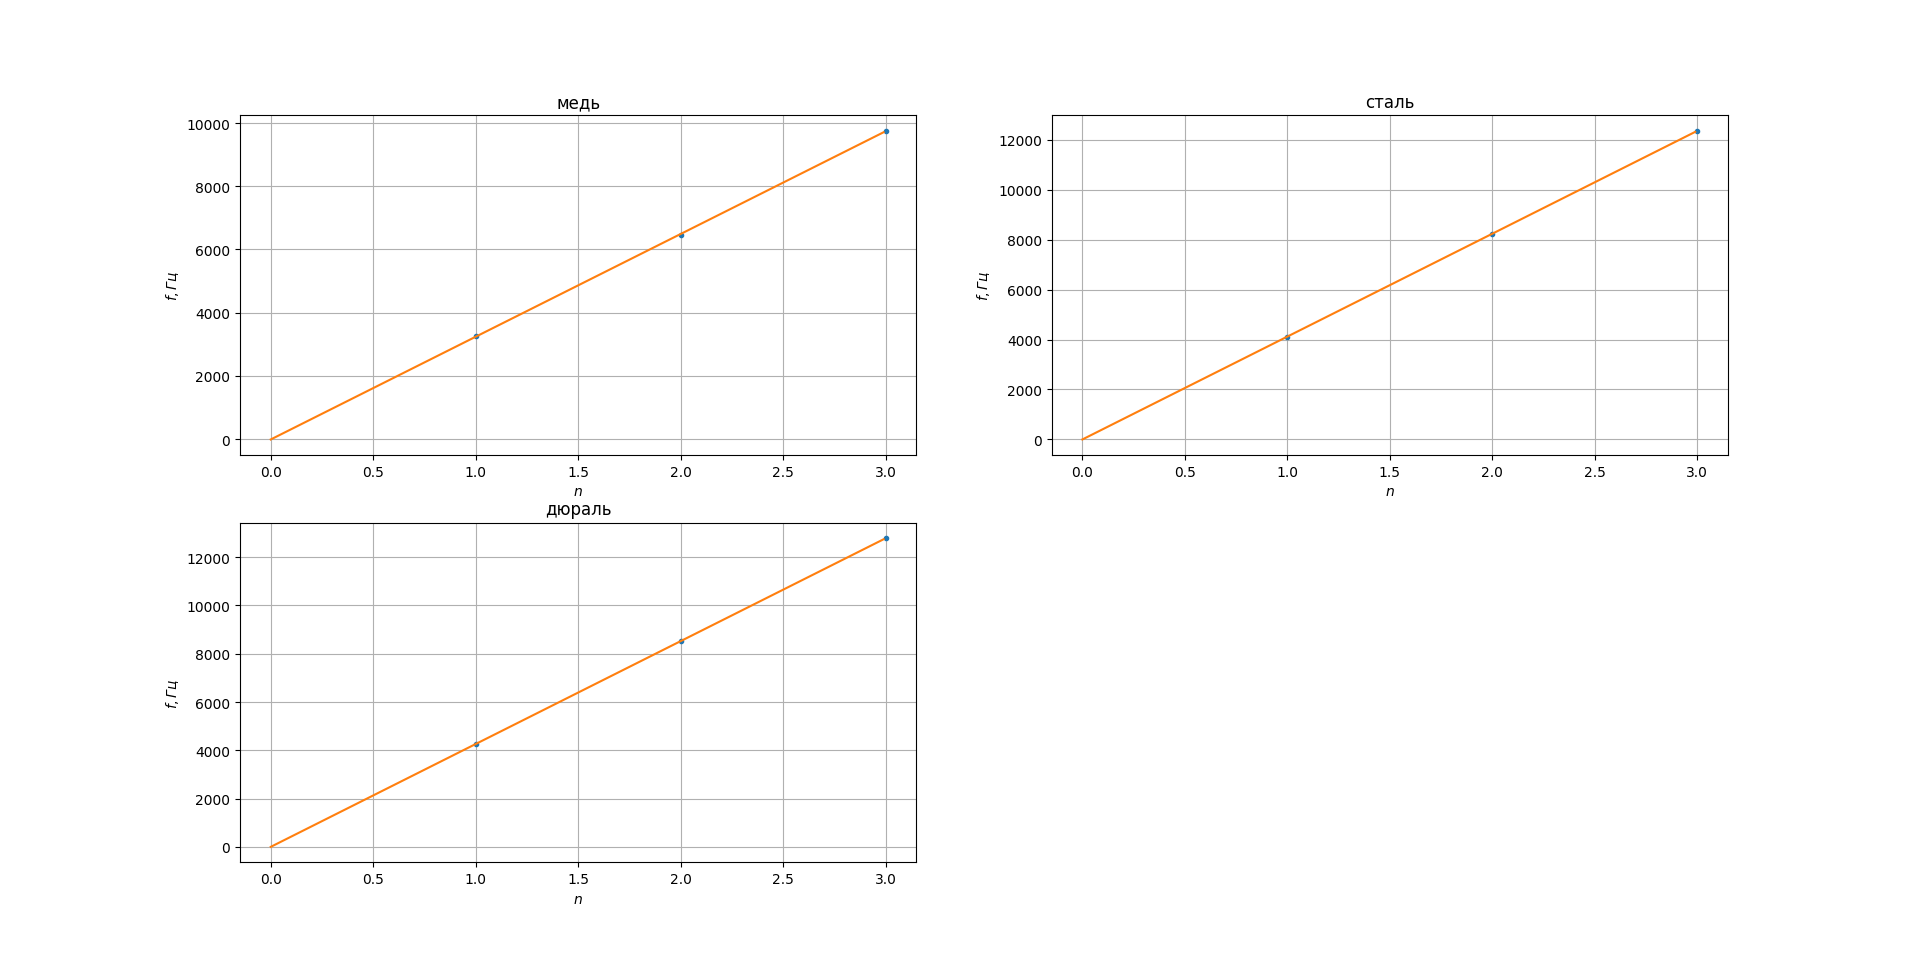
\includegraphics[width=530pt]{image/full.png}
\end{figure}

\end{document}
